\section{Introduction}
\subsection{The Explanation of Some Terms}
\rem \emph{Neurons} are highly specialized for generating electrical signals in response to chemical and other inputs, and transmitting them to other cells.
\rem \emph{Dendrites} receives information inputs from other neurons.
\rem \emph{Axon} carries the neuronal output to other cells.
\begin{center}
    \label{fig:1.1}
    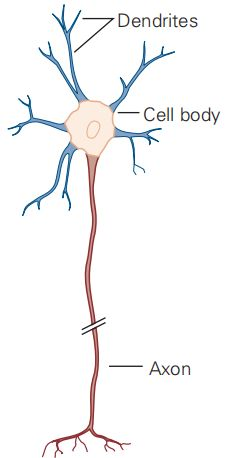
\includegraphics[scale = 0.35]{png/Figure1-1}\\
\end{center}

\rem \emph{Ion channels} control the flow of ions across the cell membrane by opening and closing in response to voltage changes and to both internal and external signals.
\begin{center}
  \label{fig:1.2}
  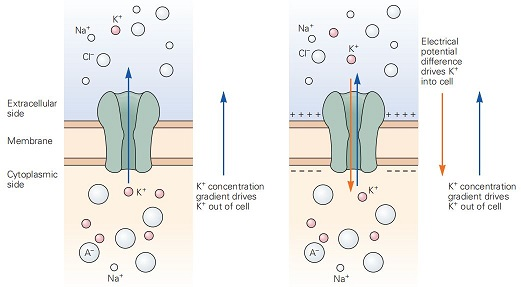
\includegraphics[scale = 0.55]{png/Figure1-2}\\
\end{center}
  
\con [Membrane Potential]The potential difference between two solutions separated by membranes, generally refers to the electrical phenomenon accompanying the life activities of cells, which exists on both side of cells.
\rem Under resting conditions,the potential inside the cell membrane(mainly K$^+$) is negative, outside the cell membrane(mainly Na$^+$) is positive, and the cell is said to be \emph{polarized}.
\defn [Action Potential] \emph{Action potential} is the characteristic electrical pulses or, more simply, spikes that can travel down nerve fibers.
\con [Hyperpolarization]Current in the form of positively charged ions flowing out of the cell (or negatively charged ions flowing into the cell) through open channels makes the membrane potential more negative, a process called \emph{hyperpolarization}.
\con [Depolarization]Current flowing into the cell changes the membrane potential to less negative or even positive values. This is called \emph{depolarization}.
\rem If a neuron is depolarized sufficiently to raise the membrane potential above a threshold level, a positive feedback process is initiated, and the neuron generates an \emph{action potential}.
\con [Absolute Refractory Period]For a few milliseconds just after an action potential has been fired, it may be virtually impossible to initiate another spike.
\con [Relative Refractory Period]After the absolute refractory period, the excitability of cells gradually recovers. After stimulation, excitement can occur, but the stimulation must be greater than the original threshold intensity.
\rem \emph{Absolute refractory period} and \emph{relative refractory period} are two basic phenomena in the process of neural response.
\subsection{Recording Neuronal Responses}
\exm Intracellular and extracellular methods for recording neuronal responses electrically
\begin{center}
    \label{fig:1.3}
    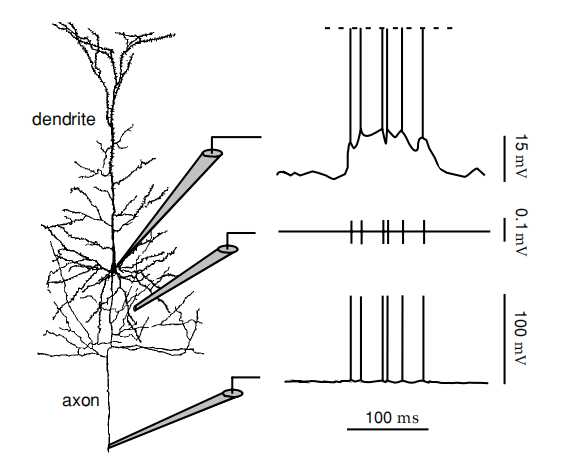
\includegraphics[scale = 0.35]{png/Figure1-3}\\
\end{center}

\begin{enumerate}[(i)]
  \item The top trace represents a recording from an intracellular electrode connected to the soma of the neuron.
  \item The middle trace is a simulated extracellular recording.
  \item The bottom trace represents a recording from an intracellular electrode connected to the axon some distance away from the soma.
\end{enumerate}




\subsection{From Stimulus to Response}
\rem  Neurons typically respond by producing complex spike sequences that reflect both the intrinsic dynamics of the neuron and the temporal characteristics of the stimulus.
\defn Neural encoding refers to the map from stimulus to response.
\exm We can catalog how neurons respond to a wide variety of stimuli, and then construct models that attempt to predict responses to other stimuli.
\defn Neural decoding refers to the reverse map, from response to stimulus.
\rem The complexity and trial-to-trial variability of action potential sequences make it unlikely that we can describe and predict the timing of each spike deterministically. Instead, we seek a model that can account for the probabilities that different spike sequences are evoked by a specific stimulus.


%%% Local Variables:
%%% mode: latex
%%% TeX-master: t
%%% End:
